\section{Artifact Description}\label{sec:artifact_description}

The selected solution to the \ac{DoHG@MHH}'s problems is the implementation of a \ac{SWfMS}: the pipeline usage will be professionalized and the optional usage of cloud services will be possible. The selection is based on the results of the literature review found in \cref{subsec:literature_review_swfms}. The following subsections will elaborately describe the artifact design and search process. All benchmarks are done with the sample \textit{NA12878} provided by the \textit{Genome in a Bottle Consortium} if not stated otherwise. The use of this sample is recommended as described in  \cref{subsection:literaturegeneticsequencing}.

\subsection{Design Search Process}
The \ac{DoHG@MHH} needs a \ac{SWfMS} that fulfills the following needs:
\begin{itemize}
    \item Support for \textit{\ac{SLURM}}, the job scheduler used by \ac{MHH}'s \ac{HPC} cluster.
    \item Support for \textit{Singularity}, the container format used by \ac{MHH}'s \ac{HPC} cluster.
    \item Support for the optional use of cloud providers (changeable per pipeline run), at least \ac{AWS}.
    \item Accessible and usable by the biologists and medical staff that currently operate the pipeline.
\end{itemize}

A \ac{GUI} based tool like \textit{Galaxy} seems promising regarding accessibility and usability. But as \citeauthor{wratten2021} \autocite{wratten2021} outline, expressiveness is lacking. Additionally, the already validated \textit{\ac{megSAP}} would have to be re-implemented and re-parameterized, which is not feasible. A flexible and \ac{DSL} based \ac{SWfMS} is needed, allowing the existing pipeline to be easily ported to the new system. \textit{Nextflow} and \textit{Snakemake} are popular and modern \acp{SWfMS} of this type. Based on the literature presented in \cref{subsec:literature_review_swfms}, \textit{Nextflow} seems to have the overall edge over \textit{Snakemake} and other tools, while satisfying all requirements. Consequently, \textit{Nextflow} is chosen as the \ac{SWfMS} to be implemented at the \ac{DoHG@MHH} to reprocess the existing sequencing data.

\subsection{Analyzation of Existing Shell Script}

The \textit{Nextflow} workflow will be based on the scripts currently in use at the \ac{DoHG@MHH}. This workflow will be iteratively refined to improve its efficiency.

The \textit{bash} script, found in \cref{lst:pipelinescriptold} (\cref{appendix:bashscript}) is written by 
Dr. rer. nat. Winfried Hofmann\,\orcidlink{0000-0001-6658-3366} of the \ac{DoHG@MHH} and was created in July 2019.

The script begins by defining several variables that will be used later in the script. The first three variables are the full path to the commands for the \lstinline{pwd} and \lstinline{mkdir} functions and the current date (lines \numrange{5}{7}). The \lstinline{pwd} command returns the current working directory, while the \lstinline{mkdir} command creates a new directory. The current date is stored in the variable \lstinline{DATE} in the format \textit{year-month-day\_seconds}. The assignment of the full path of the \lstinline{pwd} and \lstinline{mkdir} commands within the script is not necessary, as they are not utilized in a differing environment or context. Therefore, these assignments are redundant.

The script then sets three working directories (lines \numrange{10}{12}):
\begin{enumerate}
    \item The current working directory as the variable \lstinline{WDIR} using the \lstinline{pwd} command.
    \item The working directory in the \textit{Singularity} container as the variable \lstinline{WDIR_SINGULARITY} by using the \lstinline{sed} command to modify the \lstinline{WDIR} path to remove the \lstinline{/mnt/hgenet} prefix.
    \item The hard-coded \textit{\ac{SLURM}} working directory as the variable \lstinline{WDIR_SLURM}.
\end{enumerate}

The script then changes the working directory to \lstinline{WDIR} using the \lstinline{cd} command (line \num{14}). Since the current directory is still the same, this step is unnecessary, and the command will not result in any meaningful change to the current working directory.

Next, the script creates an array called \lstinline{SAMPLEDIRARRAY} of directories having names starting with \lstinline{Sample\_} using the \lstinline{ls} and \lstinline{grep} commands (line \num{15}). The \lstinline{ntasks} variable is then set to the number of directories in the array using the \lstinline{echo} command (line \num{16}). This variable is defined in the script, but it is not used in any subsequent operations, making its definition superfluous.

The script checks if a subdirectory of \lstinline{WDIR_SLURM} with the current date time combination (\lstinline{DATE}) exists. If the directory does not exist, the script creates the directory using the \lstinline{mkdir} command (lines \numrange{19}{21}). By using \lstinline{mkdir}'s parameter \lstinline{-p}, as described in \autocite{IEEEAndTheOpenGroup2018}, the complexity could be reduced by removing the conditional statement as an existing directory would be ignored without an error.

The script then enters a loop that iterates over each of the directories in the  \lstinline{SAMPLEDIRARRAY} array. For each \lstinline{SAMPLEDIR}, the script uses the \lstinline{sed} command to extract the sample ID from the directory name. The script then creates a bash file itself, with the sample ID as the name, and writes several \lstinline{SBATCH} directives to the file via the \lstinline{echo} command. \lstinline{SBATCH} directives are used to specify resources and the execution environment for jobs submitted to a \textit{\ac{SLURM}} batch system with the \lstinline{sbatch} command. When the script or command file is executed, the batch system allocates the specified resources and executes the job according to the specified execution environment. The used \lstinline{SBATCH} commands in line \numrange{28}{38} are:
\begin{description}[leftmargin=*,widest=\texttt{\#SBATCH --cpus-per-task=n}]
    \item[\texttt{\#SBATCH -J jobname}] Specifies the name of the job.
    \item[\texttt{\#SBATCH -p partition}] Specifies the partition or queue in which the job should be run.
    \item[\texttt{\#SBATCH --exclude=nodes}] Specifies a list of nodes on which the job should not be run.
    \item[\texttt{\#SBATCH --no-kill}] Specifies that the job should not be terminated when the user logs out.
    \item[\texttt{\#SBATCH --cpus-per-task=n}] Specifies the number of CPUs that should be allocated to each task of the job.
    \item[\texttt{\#SBATCH --mem=n[G|M|K]}] Specifies the amount of memory that should be allocated to the job.
    \item[\texttt{\#SBATCH --time=hh:mm:ss}] Specifies the maximum runtime of the job.
    \item[\texttt{\#SBATCH --chdir=directory}] Specifies the working directory for the job.
    \item[\texttt{\#SBATCH --error=file}] Specifies the file to which the standard error output of the job should be redirected.
    \item[\texttt{\#SBATCH --output=file}] Specifies the file to which the standard output of the job should be redirected.
\end{description}
The \lstinline{--exclude} command is given twice. This could be merged into one statement.

The \lstinline{singularity exec} command (line \num{39}), which is used to execute a command within a \textit{Singularity} container, finalizes the newly created bash file. The \lstinline{-B} option is followed by a list of directories to be bound from the host to the container file system, in the format \lstinline{host_path:container_path}. Then the path to the \textit{Singularity} container is specified. Finally, the command running the \lstinline{analyze.php} script of \textit{\ac{megSAP}} follows, with several arguments:
\begin{description}
    \item[\texttt{-folder \$WDIR\_SINGULARITY/\$SAMPLEDIR}] Specifies the working directory for the pipeline based on the previously defined variables.
    \item[\texttt{-name \$SAMPLEID}] Specifies the name of the sample based on the previously defined variable.
    \item[\texttt{-use\_dragen}] Instructs the pipeline to use the \textit{DRAGEN} systems of the \ac{DoHG@MHH}.
    \item[\texttt{-no\_abra}] Specifies to ignore the \textit{abra} part of the pipeline.
    \item[\texttt{-system /NGS\_Daten\_Test/Manifest/NGSD/IDTPanelV2\_GRCh38.tsv}] Specifies the path to the desired system manifest file.
    \item[\texttt{-threads 12}] Specifies the number of threads to use for the pipeline execution, in this case 12.
\end{description}

The loop then ends with the \lstinline{sbatch} command used to submit the job to the \textit{\ac{SLURM}} batch system using the newly created script (line \num{40}). This step is the last in the loop and concludes the pipeline script.

\textit{\ac{megSAP}} logs the execution time in a file for every processed sample. An analyzation of \num{500} random samples processed in 2022 shows that the pipeline for a genome analyzation usually runs for a little longer than a day (see \cref{table:scriptruntimestats}).

\begin{table}[H]
\centering
\caption[Descriptive statistics of \acs{megSAP} runtime for genome samples]{Descriptive statistics of \acs{megSAP} runtime for genome samples}{\num{500} random samples analyzed by the \ac{DoHG@MHH} in 2022 were analyzed.\\\smallskip}
\label{table:scriptruntimestats}
\small
\begin{tabular}{lr}
\toprule
Statistic & Duration \\
\midrule
Mean & \SI{1}{\day}, \SI{1}{\hour}, \SI{56}{\minute} \\
Standard deviation & \SI{0}{\day}, \SI{6}{\hour}, \SI{42}{\minute} \\
Median & \SI{1}{\day}, \SI{0}{\hour}, \SI{31}{\minute} \\
\bottomrule
\end{tabular}
\end{table}

\subsection{Initial Conversion to a Nextflow Workflow}\label{subsection:initialworkflow}
As a first step, the existing shell script is translated to a \textit{Nextflow} workflow as accurately as possible to ensure that no errors occur based on this initial change. The definition of the workflow consists of two files:
\begin{description}
    \item[\texttt{megsap\_germline.nf}] A script written in the \textit{Nextflow} script \ac{DSL} (Version 2) (see \cref{appendix:megsapgermlinev01}, \cref{lst:megsapgermlinev01}).
    
    The script header contains the shebang pointing to the \textit{Nextflow} interpreter (using the \textttx{env} program), and the directive to use version 2 of the \textit{Nextflow} \ac{DSL} (see \autocite{SeqeraLabs2022}) (line \numrange{1}{2}).
    
    The script begins by setting the \lstinline{sampledir} parameter to a directory that usually contains the sample data: \textttx{\$\{launchDir\}/Sample\_*} (line \num{4}). \textttx{\$\{launchDir\}} is a variable provided by \textit{Nextflow} and contains the directory where the \textttx{nextflow} command is run, \textttx{/Sample\_*} matches any directories with names starting with \textit{Sample\_}.
    
    The script then defines a process named \textttx{megSAP} (line \num{8}), which takes a single input value, \textttx{sampleDirectory}. The following \textttx{script} block (line \numrange{11}{15}) defines the commands that will be executed when that process is run. First, the directory and the sample name are derived from the given sample directory using the \textit{Nextflow} \ac{DSL}. Then the \textit{PHP} command to run \textit{\ac{megSAP}} using all relevant parameters is specified as a \textit{bash} snippet enclosed by three double-quotes.
    
    The workflow definition (line \numrange{18}{20}) introduces a channel created with the\linebreak\textttx{Channel.fromPath} command. A channel is a way to represent and manage data flow within a \textit{Nextflow} pipeline. It is a key concept which is used to define the inputs and outputs of processes, as well as to connect processes together. In this script, a channel of directory paths defined by the \textttx{sampledir} parameter is created and then piped (see \autocite[Pipes]{SeqeraLabs2022}) to the \textttx{megSAP} process as input. This means that the \textttx{megSAP} process will be executed on each directory that matches the pattern defined by the \textttx{sampledir} parameter.
    
    \item[\texttt{nextflow.config}] A \textit{Nextflow} configuration file containing the definitions of the runtime environment (see \cref{appendix:megsapgermlinev01}, \cref{lst:megsapnextflowconfigv01}).
    
    The first block of code, \textttx{process \{...\}} (line \numrange{1}{11}), sets various options for the pipeline's process. The \textttx{debug} option is set to \textttx{true}, which means that \textit{Nextflow} will output additional information, especially the standard output, to the console for debugging purposes. The executor is set to \textttx{slurm}, which means that the pipeline will use the \textit{\ac{SLURM}} job scheduler to manage the execution of the pipeline's processes. \textttx{clusterOptions} is set to a string of options passed to the \textit{\ac{SLURM}} scheduler, such as the time, partition, and nodes to exclude, and the \textttx{container} option is set to the path of the \textit{Singularity} container image that will be used to run the pipeline's processes. The \textttx{containerOptions} are additional options passed to the container to mount certain directories. The \textttx{stageInMode} is set to \textttx{'symlink'} which means that files will be symlinked into the container instead of copied. The \textttx{cache} option is set to \textttx{false}, which means that \textit{Nextflow} will not use caching for intermediately used files when between processes. The latter is not necessary, as the \textit{Nextflow} pipeline currently only contains one process step. The \textttx{cpus} option is set to \textttx{12} which means that the pipeline's processes will use 12 CPU cores. The memory option is set to \textttx{50.GB}, which means that the pipeline's processes will use \SI{50}{\giga\byte} of memory.
    
    The \textttx{singularity} block of the configuration (line \numrange{13}{16}) enables the use of \textit{Singularity} for the pipeline, and sets the \textttx{autoMounts} option to true, which means that \textit{Nextflow} will mount the file systems specified in the \textttx{containerOptions}.
    
    The \textttx{report} (line \numrange{18}{22}), \textttx{timeline} (line \numrange{24}{28}), and \textttx{dag} (line \numrange{30}{34}) blocks of code enable the generation of various reports for the pipeline (see \autocite{SeqeraLabs2022a}) such as the HTML execution report, an HTML timeline report and a visualization of the pipeline's \ac{DAG} respectively. The \textttx{file} option is set to the desired file names of the reports and the \textttx{overwrite} option is set to true, which means that \textit{Nextflow} will overwrite the report file if it already exists.
    
    Finally, the \textttx{cleanup} option is set to {true} (line \num{36}), which means that \textit{Nextflow} will remove intermediate files and directories when the pipeline completes.
\end{description}

This split into two files leans on the design principle \enquote{separation of concerns}, as the functional workflow itself is split from the definition of the environment it is run in. This principle, generally used to describe the separation of software modules (see \autocite{Parnas1972}), can be applied here as well.

Running the pipeline generates the simple \ac{DAG} depicted in \cref{fig:dag_v01}.

\begin{figure}[H]
    \centering
	\includegraphics[scale=0.8]{flowcharts/nextflow_dag_v0.1}
	\caption{\Ac{DAG} for initial Nextflow workflow}
	\label{fig:dag_v01}
\end{figure}

Running the pipeline under ideal conditions, i.e., no other jobs running on the cluster, the pipeline runs for \SI{11.5}{\hour}. Usually, this takes longer on average when multiple jobs are running (like the 48 samples processed by the sequencer), as the mapping on the \ac{DoHG@MHH}'s two \textit{DRAGEN} servers is running single threaded by design. The average CPU usage is \SI{24.5}{\percent} of the allocated \num{12} CPU cores as shown in \cref{figure:pipeline_benchmark_CPU_v01}. Peak memory usage is \SI{81.1}{\percent} of the assigned \SI{50}{\giga\byte} as shown in  \cref{figure:pipeline_benchmark_memory_v01} (see \cref{appendix:megsapgermlinev01}, \cref{table:megsapgermlinev01benchmark} for the exact values reported by \textit{Nextflow}).

\begin{figure}[H]
    \centering
	\includegraphics[width=\linewidth,height=\textheight,keepaspectratio]{pipeline_benchmark_CPU_v01}
	\caption{Average CPU usage of the initial Nextflow workflow}{Detailed statistics are listed in \cref{table:megsapgermlinev01benchmark}.}
	\label{figure:pipeline_benchmark_CPU_v01}
\end{figure}

\begin{figure}[H]
    \centering
	\includegraphics[width=\linewidth,height=\textheight,keepaspectratio]{pipeline_benchmark_memory_v01}
	\caption{Peak memory usage of the initial Nextflow workflow}{Detailed statistics are listed in \cref{table:megsapgermlinev01benchmark}.}
	\label{figure:pipeline_benchmark_memory_v01}
\end{figure}

\subsection{BAM to FastQ Conversion}

The \ac{DoHG@MHH} stores its archival data in the BAM file format described by \citeauthor{Li2009} \autocite{Li2009}. These are generated after the alignment to a reference genome. Hence, the files must be converted back to an unaligned state in the FastQ file format, outlined by \citeauthor{Cock2009} \autocite{Cock2009}, before they can be realigned to the new reference genome. This transformation will be added to the \textit{Nextflow} workflow as an optional processing step. 

\subsubsection{Evaluation of BAM to FastQ Tools}\label{subsubsec:bam2fastqeval}

Four suitable tools have been identified by a literature research and are being evaluated:
\begin{description}
    \item[biobambam2] Based on \textit{biobambam} by \citeauthor{Tischler2014} released in 2014. Not as actively maintained as the other tools (latest release March 17, 2021) and lacks documentation, but is nevertheless taken into consideration because of promising benchmark results documented in \autocite{Tischler2014}. \textit{biobambam2} does not support multithreading and is written in \textit{C++}.
    \item[ngs-bits] Released in 2015, actively maintained (latest release July 8, 2022) by the \textit{Institute of Medical Genetics and Applied Genomics at University Hospital and Faculty of Medicine T\"ubingen} \autocite{Sturm2018}. \textit{ngs-bits} does not support multithreading and is written in \textit{C++}.
    \item[Picard] Released in 2009, actively maintained (latest release June 29, 2022) by the \textit{Broad Institute of MIT and Harvard}, a non-profit biomedical and genomic research center \autocite{BroadInstitute2019}. \textit{Picard} supports multithreading and is written in \textit{Java}. It produces uncompressed FastQ files, which then require compression before further use.
    \item[SAMtools] Released in 2009, actively maintained (latest release September 2, 2022) by the \textit{Genome Research Ltd.}, a non-profit British genomics and genetics research institute \autocite{Danecek2021}. \textit{SAMtools} supports multithreading and is written in \textit{C}. BAM files need to be sorted before being converted back to the FastQ format.
\end{description}

All tools are assessed by processing a BAM file produced of a whole exome sequencing run analyzed by the \ac{DoHG@MHH} in August 2022 with a size of \SI{8.6}{\giga\byte} (see \cref{table:bam2fastq_benchmark_sample_stats} for the files statistics). This file is randomly selected and used to benchmark the performance using single- and (if possible) multithreaded (four threads) approaches. Every tool/threading combination is run ten times to ensure a representative result. To verify that the results translate to larger whole genome BAM files, each of the tools is also tested on a file from August 2022 with a size of \SI{58}{\giga\byte} (see \cref{table:bam2fastq_benchmark_sample_stats} for the files statistics). Given that the results are transferable, only a single run is conducted due to time restraints. The benchmarks are run on a virtual machine equipped with 4 CPUs (Intel\textsuperscript{\textregistered} Xeon\textsuperscript{\textregistered} Gold 6148 processor with \SI{2.40}{\giga\hertz}) and \SI{8}{\giga\byte} RAM. 

The main factor relevant for the valuation of the tools is the duration of the conversion. As seen in \cref{figure:bam2fastqbenchmarkruntime}, \textit{ngs-bits} is the fastest. Secondary factors, the amount of memory (see \cref{figure:bam2fastqbenchmarkmemory}) and data read/written on disk (see \cref{figure:bam2fastqbenchmarkio}), do favor \textit{ngs-bits} as well (only \textit{biobambam2} uses less memory which is negligible). Due to the already poor performance in multithreading mode, \textit{Picard} was not tested single threaded. Multithreading capabilities do not play a relevant role in the consideration of the tool to be used: multiple single threaded conversions may be run in parallel, depending on the number of cores available on the device used and the number of files to be processed. As \textit{ngs-bits} is already used by \textit{\ac{megSAP}}, this tool will also not introduce an additional dependency.

As expected, conversions with a genome file took longer, but with similar relative time differences between the tools (see \cref{figure:bam2fastqbenchmarkruntimegenome}).

Based on this results, \textit{ngs-bits} is used for conversions of BAM to FastQ files.

\begin{figure}[H]
    \centering
	\includegraphics[width=\linewidth,height=\textheight,keepaspectratio]{bam2fastqbenchmark_runtime}
	\caption[Median duration of BAM to FastQ conversion of whole exome data by tool]{Median duration of BAM to FastQ conversion of whole exome data by tool}{Detailed statistics are listed in \cref{table:bam2fastqduration}.}
	\label{figure:bam2fastqbenchmarkruntime}
\end{figure}

\begin{figure}[H]
    \centering
	\includegraphics[width=\linewidth,height=\textheight,keepaspectratio]{bam2fastqbenchmark_memory}
	\caption[Median memory usage of BAM to FastQ conversion of whole exome data by tool]{Median memory usage of BAM to FastQ conversion of whole exome data by tool}{Detailed statistics are listed in \cref{table:bam2fastqmemory}.}
	\label{figure:bam2fastqbenchmarkmemory}
\end{figure}

\begin{figure}[H]
    \centering
	\includegraphics[width=\linewidth,height=\textheight,keepaspectratio]{bam2fastqbenchmark_io}
	\caption[Median amount of data read and written by BAM to FastQ conversion of whole exome data by tool]{Median amount of data read and written by BAM to FastQ conversion of whole exome data by tool}{Detailed statistics are listed in \cref{table:bam2fastqioread,table:bam2fastqiowrite}.}
	\label{figure:bam2fastqbenchmarkio}
\end{figure}

\begin{figure}[H]
    \centering
	\includegraphics[width=\linewidth,height=\textheight,keepaspectratio]{bam2fastqbenchmark_runtime_genome}
	\caption[Duration of BAM to FastQ conversion of whole genome data by tool]{Duration of BAM to FastQ conversion of whole genome data by tool}{Detailed statistics are listed in \cref{table:bam2fastqdurationgenome}.}
	\label{figure:bam2fastqbenchmarkruntimegenome}
\end{figure}

\subsubsection{Integration of BAM to FastQ Tool into Nextflow Workflow}

To add the optional BAM to FastQ conversion to the \textit{Nextflow} workflow, both, the workflow definition (see \cref{appendix:megsapgermlinev02}, \cref{lst:megsapgermlinev02}) and the configuration (\cref{lst:megsapnextflowconfigv02}), need to be modified.

A process definition, \textttx{bam2FastQ}, is added to the workflow (line \numrange{6}{25}). The process uses a single input variable, the \textttx{sampleDirectory} containing a BAM file as input (line \num{8}). Two output variables are defined: The first one is a \textttx{path} channel for the generated FastQ files emitted as \textttx{fastq} (line \num{11}). This ensures that \textit{Nextflow} picks up the files and moves them to the sample directory, as later specified by the \textttx{publishDir} directive (line \num{14}). This mechanism was not used before, as \textit{\ac{megSAP}} outputs all files to the sample directory by itself. The second output variable is the passed through \textttx{sampleDirectory} variable, which is emitted through a channel named \textttx{sampledir} (line \num{12}). The process script extracts the sample name from the directory path (line \num{17}), and uses the \textttx{files()} function to find the first BAM file in the \textttx{sampleDirectory} (line \num{18}). Next, the process runs a command that calls the \textit{ngs-bits} \textttx{BamToFastq} script (line \numrange{20}{23}), passing the BAM file path and the output files location and names as arguments.

To allow for BAM or FastQ file input for the pipeline, two channels are defined in the workflow part: \textttx{bam\_channel} and \textttx{fastq\_channel}. The \textttx{bam\_channel} is created using the \textttx{Channel.fromPath()} function, which takes a path specified in the \textttx{params.sampledir} variable, and maps the input directories using a closure that filters the directories that contain at least one BAM file and no FASTQ files (line \numrange{40}{44}). Then the \textttx{bam2FastQ} process is applied to the \textttx{bam\_channel} (line \num{45}). The \textttx{fastq\_channel} is also created using the \textttx{Channel.fromPath()} function, and maps the input directories using a closure that filters the directories that contain no BAM files and at least two FASTQ files (line \numrange{47}{51}). Finally, the \textttx{fastq\_channel} is mixed with the \textttx{sampledir} output of the \textttx{bam2FastQ} process (the passed-through directory of the processed sample) and used as input to the \textttx{megSAP} process (line \num{53}).

The used \textttx{mix} operator of the \textit{Nextflow} \ac{DSL} creates a channel containing all the elements of the original channels, in the order they were presented, as described in \autocite{SeqeraLabs2022b}. This allows the pipeline to start processing samples already in the FastQ file format to be processed with \textit{\ac{megSAP}} without waiting for other samples to be converted from the BAM file format.

To use \textit{Nextflow}'s features for staging and moving files as defined by the \textttx{bam2FastQ} process, data paths have to be the same in- and outside the container, as noted in \autocite{SeqeraLabs2022c}. Thus, the bind paths definition has been appended with one-to-one mappings of the local file system in the configuration file (line \num{6}). As presented in \cref{subsubsec:bam2fastqeval}, the \textttx{BamToFastq} command of \textit{ngs-bits} does not need as many resources as currently defined for the whole workflow. Hence, an exclusion for the \textttx{bam2FastQ} process is introduced (line \numrange{11}{14}), limiting the process to \num{2} CPU cores and \SI{8}{\giga\byte} of memory.

The new additions lead to a slightly more complex \ac{DAG}, as shown in \cref{fig:dag_v02}. The link from the generated FastQ files to \textit{\ac{megSAP}} has been added to the diagram manually, as \textit{Nextflow} is not aware of the data flow. The files are simply present in the directory \textit{\ac{megSAP}} runs in.

\begin{figure}[H]
    \centering
	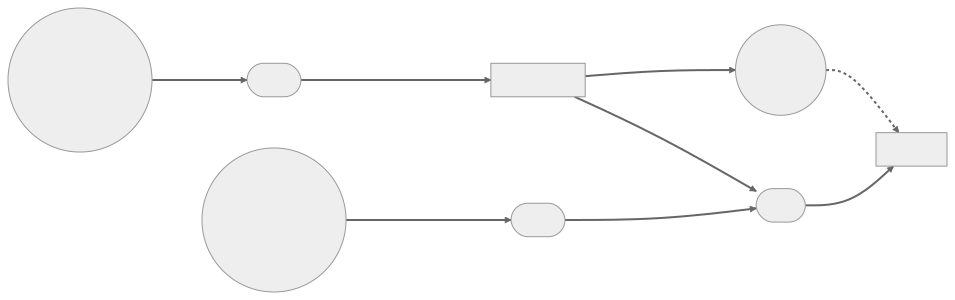
\includegraphics[scale=0.8]{flowcharts/nextflow_dag_v0.2}
	\caption{\Ac{DAG} for Nextflow workflow with added BAM to FastQ file conversion}
	\label{fig:dag_v02}
\end{figure}

An evaluation of the combined workflow is not conducted, as results can be derived from the previous measurements: a genome analysis will take about \SI{1.65}{\hour} longer with BAM to FastQ conversion.

\subsection{Separation of \acs{megSAP} Steps}\label{subsection:seperationofsteps}

To optimize \textit{\ac{megSAP}}'s resource usage, the individual steps \textemdash mapping, variant calling, copy number variant calling, structural variant calling, and database import (see \cref{fig:flowchart_overview}) \textemdash need to be separated. After splitting, each step can be measured on its own by \textit{Nextflow}'s build in HTML execution report (see \autocite{SeqeraLabs2022a}). To accomplish this, the \textit{Nextflow} process \textttx{megSAP} is replaced by five separate processes (\cref{lst:megsapgermlinev03}, line \numrange{27}{100}): \textttx{megSAPma}, \textttx{megSAPvc}, \textttx{megSAPcn}, \textttx{megSAPsv}, and \textttx{megSAPdb}. These processes are nearly identical to the \textttx{megSAP} process in the last iteration, with three changes:
\begin{enumerate}
    \item The variable \textttx{threads} containing the number of threads defined in the \textit{Nextflow} configuration file (e.g., line 39).
    \item The variable \textttx{steps} defining the steps to be run during the execution of \textit{\ac{megSAP}} (e.g., line 40). This variable is the only difference between the newly added process blocks.
    \item The command to call \textit{\ac{megSAP}} has been extracted to a separate script (see \cref{lst:megsapgermlinesh}) in a template folder. The \textttx{template} keyword (e.g., line 41) is used to define a reusable code fragment that can be utilized in multiple places within a workflow. Templates can be parameterized, allowing different values to be passed in each time the template is used, in this case the previous introduced parameters \textttx{containerDirectory} and \textttx{sampleName} accompanied by the new \textttx{threads} and \textttx{steps}. Templates provide a way to factor out common parts of a pipeline and simplify pipeline development, making the code more readable and maintainable. By utilizing this part of \textit{Nextflow}'s \ac{DSL} described in \autocite[Module templates]{SeqeraLabs2022}, this common data processing operation can be shared across all processes calling \textit{\ac{megSAP}}.
\end{enumerate}
Creating multiple process steps instead of implementing a reusable process with a calling parameter to set the \textit{\ac{megSAP}} step is deliberate. Resource allocation in the configuration can only be done by providing the process name or adding a label to a process. Both cannot be changed dynamically. So the goal, setting different resource constraints for each step, cannot be reached without creating multiple process blocks.

The separation shows a direct flow between the consecutive steps in the generated \ac{DAG}, as seen in \cref{fig:dag_v03}.

\begin{figure}[H]
    \centering
	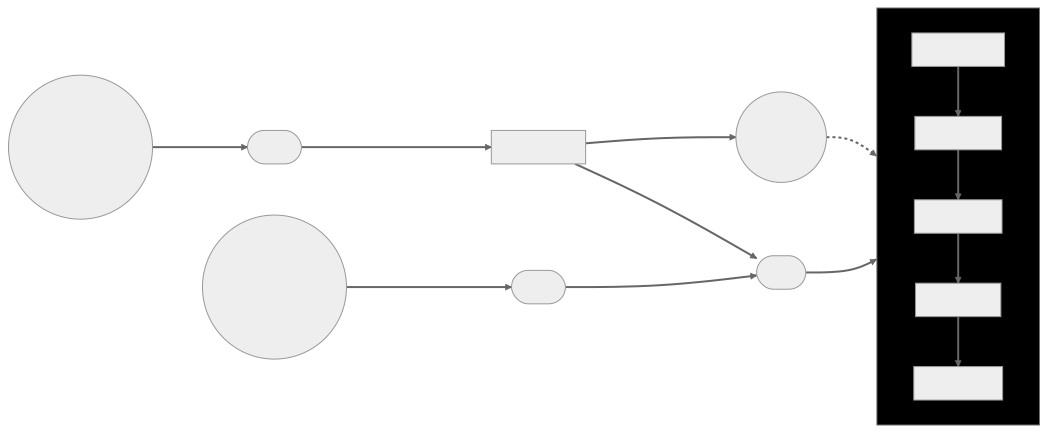
\includegraphics[width=1\textwidth,height=0.9\textheight,keepaspectratio]{flowcharts/nextflow_dag_v0.3}
	\caption{\Ac{DAG} for Nextflow workflow after separation of \acs{megSAP} steps}
	\label{fig:dag_v03}
\end{figure}

The separated workflow ran for approximately \SI{12.9}{\hour} (see \cref{table:megsapgermlinev03benchmark}). This is a little longer than the run without the split. This slight variance is expected, as other process are running on the \ac{HPC} cluster that may have an impact on file read, file write and network performance, and are not controllable. As shown previously in \cref{table:scriptruntimestats}, the standard deviation of pipeline runs in the past was \SI{6.7}{\hour}, well above the observed \SI{1.4}{\hour}. A runtime comparison between all iterations can be found in \cref{subsection:resourceoptimization}, \cref{figure:pipeline_benchmark_runtime}.

The average CPU utilization for each process varies substantially, with the highest utilization being \SI{53.1}{\percent} for the \textttx{megSAPvc} process and the lowest being \SI{1.7}{\percent} for the \textttx{megSAPdb} process as shown in \cref{figure:pipeline_benchmark_CPU_v03}. The peak memory usage also varies significantly among the processes, ranging from \SI{2}{\percent} for the \textttx{megSAPma} process to \SI{81.9}{\percent} for the \textttx{megSAPcn} process, as shown in \cref{figure:pipeline_benchmark_memory_v03}. A representation of the CPU and memory allocation and usage over time can be seen in \cref{figure:pipeline_benchmark_CPU_aoc_v03,figure:pipeline_benchmark_memory_aoc_v03}. Detailed statistics are listed in \cref{table:megsapgermlinev03benchmark}.

\begin{figure}[H]
    \centering
	\includegraphics[width=\linewidth,height=\textheight,keepaspectratio]{pipeline_benchmark_CPU_v03}
	\caption{Average CPU usage of the Nextflow workflow after separation of steps}
	\label{figure:pipeline_benchmark_CPU_v03}
\end{figure}

\begin{figure}[H]
    \centering
	\includegraphics[width=\linewidth,height=\textheight,keepaspectratio]{pipeline_benchmark_memory_v03}
	\caption{Peak memory usage of the Nextflow workflow after separation of steps}
	\label{figure:pipeline_benchmark_memory_v03}
\end{figure}

\begin{figure}[H]
    \centering
	\includegraphics[width=\linewidth,height=\textheight,keepaspectratio]{pipeline_benchmark_CPU_v3_aoc}
	\caption{Average CPU usage of the Nextflow workflow over time after separation of steps}
	\label{figure:pipeline_benchmark_CPU_aoc_v03}
\end{figure}

\begin{figure}[H]
    \centering
	\includegraphics[width=\linewidth,height=\textheight,keepaspectratio]{pipeline_benchmark_memory_v3_aoc}
	\caption{Memory usage of the Nextflow workflow over time after separation of steps}
	\label{figure:pipeline_benchmark_memory_aoc_v03}
\end{figure}

\subsection{Resource Optimization of \acs{megSAP} Steps}\label{subsection:resourceoptimization}

Based on the reported resource usage after the separation of the \textit{\ac{megSAP}} steps, each process is set up with its own resource directives within the \textit{Nextflow} configuration. This is being realized with the \textttx{withName} process selector described in \autocite[Process selectors]{SeqeraLabs2022e}. These allow to set specific parameters only for processes with a particular name. The values themselves are derived from the results shown previously in \cref{figure:pipeline_benchmark_CPU_v03} and \cref{figure:pipeline_benchmark_memory_v03}. This cannot be done as precisely as needed for the CPU requirements, as \textit{Nextflow} measures the weighted average of CPU utilization (see \autocite{SeqeraLabs2022d}). Therefore, a little buffer is added to the CPU allocation. Additionally, the mapping step (\textttx{ma}) has an outstanding characteristic: within this step, \textit{\ac{megSAP}} utilizes two \textit{Illumina DRAGEN} servers (see \autocite{IlluminaInc.2022}) owned by the \ac{DoHG@MHH}. These operate outside the \textit{SLURM} cluster in their own \textit{Sun Grid Engine} environment. Each can process one sample at a time. The external child process is not monitored by \textit{Nextflow}, as \textit{\ac{megSAP}} itself is just idly waiting. This dilutes the CPU related measurements of this step, as it also includes the usage of \textit{SeqPurge} to optimize the data before mapping takes place as described in \autocite{Sturm2016}. That part of the mapping step is best run using 15 threads (see \cref{appendix:correspondecemarc}) resulting in this being set as a configuration parameter. Each process step is also configured with a small buffer of \SI{10}{\percent} (and rounded up to the next even number) to factor in some fluctuation. 

The resulting configuration values are shown in \cref{table:resourceoptimization} and can be seen in the updated configuration in \cref{lst:megsapnextflowconfigv04}.

With this configuration, the pipeline ran for \SI{13.6}{\hour}. See \cref{figure:pipeline_benchmark_runtime} for a comparison between the runtime of all pipeline configurations.

\begin{table}[H]
\centering
\caption{Configured resource allocation after optimization}
\label{table:resourceoptimization}
    \begin{tabularx}{\textwidth}{lYYYYY}
        \toprule
        process & megSAPma & megSAPvc & megSAPcn & megSAPsv & megSAPdb \\ 
        \midrule
        allocated CPUs & \num{15} & \num{8} & \num{2} & \num{2} & \num{2} \\ 
        allocated memory & \SI{2}{\giga\byte} & \SI{20}{\giga\byte} & \SI{48}{\giga\byte} & \SI{2}{\giga\byte} & \SI{2}{\giga\byte} \\
        \bottomrule
    \end{tabularx}
\end{table}

\begin{figure}[H]
    \centering
	\includegraphics[width=\linewidth,height=\textheight,keepaspectratio]{pipeline_benchmark_runtime_v04}
	\caption{Comparison of pipeline runtime over all iterations}
	\label{figure:pipeline_benchmark_runtime}
\end{figure}

The CPU usage of the \textttx{megSAPvc} and \textttx{megSAPcn} steps is decreased, although they still do not use all allocated cores efficiently as shown in \cref{figure:pipeline_benchmark_CPU_v04}. This applies especially to the \textttx{megSAPma} step, but was expected, as described before. Memory usage is reduced in the \textttx{megSAPvc} and \textttx{megSAPcn} steps as well, with the latter not even using half its provided memory resources, as shown in \cref{figure:pipeline_benchmark_memory_v04}. A representation of the CPU and memory allocation and usage of the optimized workflow over time can be seen in \cref{figure:pipeline_benchmark_CPU_aoc_v04,figure:pipeline_benchmark_memory_aoc_v04}. Detailed statistics are listed in \cref{table:megsapgermlinev04benchmark}.

\begin{figure}[H]
    \centering
	\includegraphics[width=\linewidth,height=\textheight,keepaspectratio]{pipeline_benchmark_CPU_v04}
	\caption{Average CPU usage of the Nextflow workflow after optimization}
	\label{figure:pipeline_benchmark_CPU_v04}
\end{figure}

\begin{figure}[H]
    \centering
	\includegraphics[width=\linewidth,height=\textheight,keepaspectratio]{pipeline_benchmark_memory_v04}
	\caption{Peak memory usage of the Nextflow workflow after optimization}
	\label{figure:pipeline_benchmark_memory_v04}
\end{figure}

\begin{figure}[H]
    \centering
	\includegraphics[width=\linewidth,height=\textheight,keepaspectratio]{pipeline_benchmark_CPU_v4_aoc}
	\caption{Average CPU usage of the Nextflow workflow after optimization over time}
	\label{figure:pipeline_benchmark_CPU_aoc_v04}
\end{figure}

\begin{figure}[H]
    \centering
	\includegraphics[width=\linewidth,height=\textheight,keepaspectratio]{pipeline_benchmark_memory_v4_aoc}
	\caption{Memory usage of the Nextflow workflow after optimization over time}
	\label{figure:pipeline_benchmark_memory_aoc_v04}
\end{figure}

\subsection{Resilience and Monitoring}\label{subsection:resilienceandmonitoring}

To make the pipeline less prone to errors, two of \textit{Nextflow}s directives for error handling are introduced to the process configuration (see \cref{appendix:megsapgermlinev1}, \cref{lst:megsapnextflowconfigv1}):
\begin{description}
    \item[\textttx{maxRetries}] This option sets the maximum number of times a task will be re-executed in case of failure (see \autocite[Directives/maxRetries]{Seqeralabs2022f}. This is set to \textttx{2} (line \num{12}).
    \item[\textttx{errorStrategy}] This directive provides the capability to specify how an error should be handled by the process (see \autocite[Directives/errorStrategy]{Seqeralabs2022f}. By default, if an error status is returned by the executed script, the process immediately stops, leading to termination of the entire pipeline. This \textttx{errorStrategy} is called \textttx{terminate}. Other options are:
    \begin{description}[leftmargin=*,widest=ignore]
        \item[\textttx{finish}] Activates a controlled shutdown of the pipeline in response to an error event, while allowing the execution of any submitted tasks to complete.
        \item[\textttx{ignore}] Ignores any execution errors during the process.
        \item[\textttx{retry}] Restarts a process that returns an error condition.
    \end{description}
    To retry a process step after an error, the \textttx{retry} option is chosen. This option falls back to the \textttx{terminate} option if the maximum defined number of retries is reached. If multiple samples are analyzed in one execution of the \textit{Nextflow} workflow, this is not desired, as other samples might process without any errors. Thus, a dynamic approach of setting the \textttx{errorStrategy} is employed, setting the option to \textttx{ignore} in the event of a failed second execution attempt (line \num{13}).
\end{description}

Connecting \textit{Nextflow} to an email server allows for automatic notifications for pipeline completion, whether successful or with errors (see \autocite[Scope mail]{SeqeraLabs2022e}). This is set up in line \numrange{63}{67}.

An evaluation of these changes is not needed, as those neither affect resource consumption nor runtime.